
\documentclass{beamer}

\mode<presentation> {

% The Beamer class comes with a number of default slide themes
% which change the colors and layouts of slides. Below this is a list
% of all the themes, uncomment each in turn to see what they look like.
\usepackage{listings}
\lstset{
    breaklines=true,
    basicstyle=\ttfamily\small,
    columns=flexible,
}

\usetheme{PaloAlto}


% As well as themes, the Beamer class has a number of color themes
% for any slide theme. Uncomment each of these in turn to see how it
% changes the colors of your current slide theme.

%\usecolortheme{albatross}
%\usecolortheme{beaver}
%\usecolortheme{beetle}
%\usecolortheme{crane}
%\usecolortheme{dolphin}
%\usecolortheme{dove}
%\usecolortheme{fly}
%\usecolortheme{lily}
%\usecolortheme{orchid}
%\usecolortheme{rose}
%\usecolortheme{seagull}
%\usecolortheme{seahorse}
%\usecolortheme{whale}
%\usecolortheme{wolverine}

%\setbeamertemplate{footline} % To remove the footer line in all slides uncomment this line
%\setbeamertemplate{footline}[page number] % To replace the footer line in all slides with a simple slide count uncomment this line

%\setbeamertemplate{navigation symbols}{} % To remove the navigation symbols from the bottom of all slides uncomment this line
}

\usepackage{graphicx} % Allows including images
\usepackage{booktabs} % Allows the use of \toprule, \midrule and \bottomrule in tables
\setbeamertemplate{bibliography item}{\insertbiblabel}
%----------------------------------------------------------------------------------------
%	TITLE PAGE
%----------------------------------------------------------------------------------------

\title[PID in UAVs]{APPLICATION OF UNMANNED AIRCRAFT
PID CONTROL SYSTEM FOR ROLL, PITCH
AND YAW STABILITY ON FIXED WINGS} 

\author[Sooraj Krishna S]{Sooraj Krishna S\\Reg.No. TVE25EL064}


\institute[CET] % Your institution as it will appear on the bottom of every slide, may be shorthand to save space
{
College of Engineering Trivandrum \\ % Your institution for the title page
}
\date{\today} % Date, can be changed to a custom date

\begin{document}

\begin{frame}
\titlepage % Print the title page as the first slide
\end{frame}

\begin{frame}
\frametitle{Overview} % Table of contents slide, comment this block out to remove it
\tableofcontents % Throughout your presentation, if you choose to use \section{} and \subsection{} commands, these will automatically be printed on this slide as an overview of your presentation
\end{frame}

%------------------------------------------------
\section{UAV Control}
%------------------------------------------------

\subsection{Introduction}

\begin{frame}
\frametitle{UAV Control using PID}
2 Types of Controls – 
Manual remote control from the ground, OR Self-control thru system embedded in the system\\~\\
Main Problem to tackle in both the systems – Controlling the stability of the UAV, Stabilizing it against forces of nature, wind disturbances. \\~\\ 
The UAV can measure its own Pitch, Yaw and Roll thru gyroscope acclerometers and Gryometers, And the pilot on ground can correct it or the UAV can correct it itself.\\~\\
But at large distances, delay of these measurements and pilot’s reaction time may be too late for a correction within time and may lead to a crash. Hence its necessary for both of the UAVs to be stabilised by itself.

\end{frame}
%------------------------------------------------
\subsection{Pitch, Yaw, Roll}
\begin{frame}
\frametitle{Pitch, Yaw, Roll}
\begin{table}
\centering
\begin{tabular}{p{2cm} p{4cm} p{3cm}}
\toprule
\textbf{Motion} & \textbf{Hover (VTOL) Mode} & \textbf{Forward Flight Mode}\\
\midrule
Pitch  & Differential Rotor Tilt  & Elevators  \\
Roll   & Differential Thrust  & Ailerons \\
Yaw    & Opposite Nacelle Tilt  & Rudder  \\
Thrust & Vertical Lift  & Horizontal Propulsion \\
\bottomrule
\end{tabular}
\caption{Control of pitch, yaw and roll}
\end{table}
\end{frame} 

\section{PID Controller}
%------------------------------------------------

\subsection{Introduction}
%------------------------------------------------
\begin{frame}
\frametitle{PID Controller}
Out of the various Control Systems, we are taking a look into the PID controller

\begin{block}{P - Propotional}
Propotional - Adjusts the control signal based on the magnitude of current deviation to reduce it quickly

\end{block}

\begin{block}{I – Intergral}
Intergral - Accumulates deviations over time to eliminate static errors

\end{block}

\begin{block}{D – Diiferential}
Diiferential - redicts future deviation trends to add correction signals in advance

\end{block}
\end{frame}

%------------------------------------------------
\begin{frame}
\frametitle{PID Controller System}
\begin{figure}
    \centering
    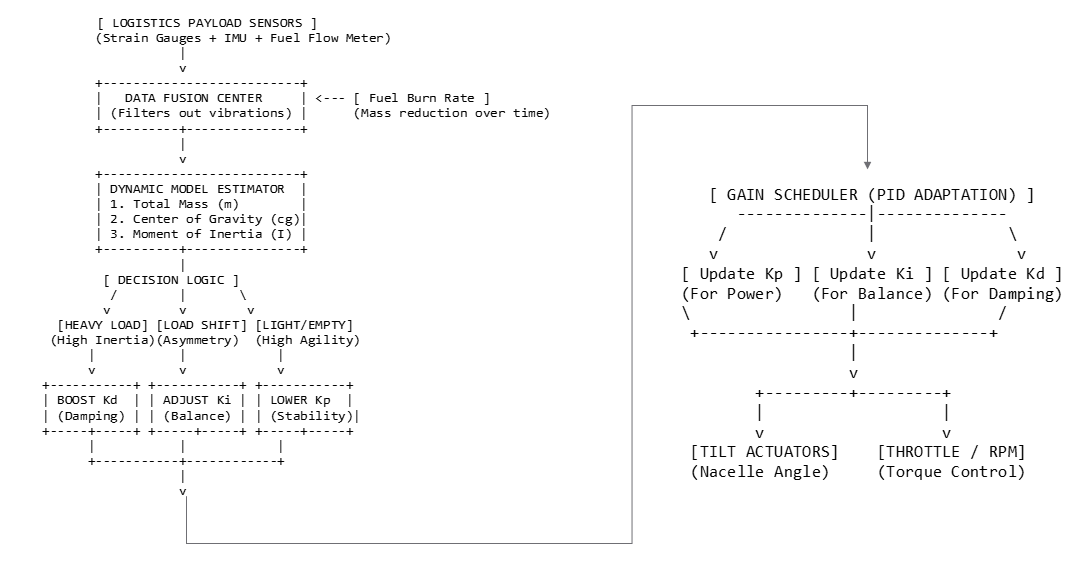
\includegraphics[width=1\linewidth]{pid1.png}
    \caption{PID Controller Flowchart}
    \label{fig:pid_controller}
\end{figure}
\end{frame}
%------------------------------------------------
\subsection{Types of PID}
\begin{frame}
\frametitle{Types of PID}
\begin{itemize}
\item \textbf{Fuzzy PID Control:} Rule-based and model-free; adjusts PID gains in real time based on conditions like payload and wind, suitable for logistics.
\item \textbf{Neural Network PID:} Learns and adapts to nonlinear flight dynamics during operation, enabling control under varying payload weights.
\item \textbf{Expert PID Control:} Uses stored expert knowledge to select optimal PID parameters for specific flight states, such as swinging cargo.
\item \textbf{Genetic Algorithm PID:} Optimizes PID parameters during the design phase using evolutionary techniques, ensuring robustness for different load weights.

\end{itemize}
\end{frame}
%------------------------------------------------

\subsection{Algorithm of PID}

\begin{frame}
\frametitle{PID Controller Algorithm}
\begin{columns}[c] % The "c" option specifies centered vertical alignment while the "t" option is used for top vertical alignment

\column{.45\textwidth} % Left column and width
\textbf{Flow of Control}
\begin{enumerate}
\item Error is the difference between setpoint and actual value.
\item PID uses P, I, and D actions for control.
\item IMU feedback enables continuous correction.
\item Proportional output scales with error via \(K_p\).
\end{enumerate}

\column{.5\textwidth} % Right column and width
\begin{figure}
    \centering
    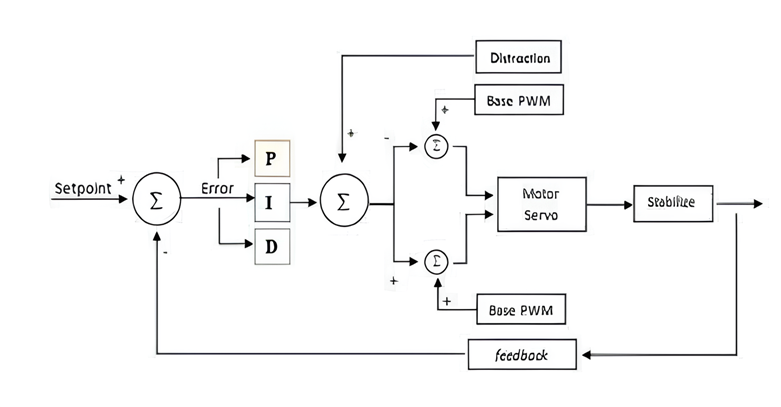
\includegraphics[width=1\linewidth]{pid2.png}
    \caption{PID Controller Algorithm}
    \label{fig:pid_algorithm}
\end{figure}

\end{columns}
\end{frame}

%------------------------------------------------
\subsection{Equations of PID}


%------------------------------------------------

\begin{frame}
\frametitle{Equation for PID Controller Algorithm : Proportional}
If $e(t)$ is the error function wrt. time.
\begin{theorem}[Propotional $K_p$]
$P=K_p e(t)$
\end{theorem}
\begin{theorem}[Integral $K_i$]
$I = K_i \int_{0}^{t} e(t)dt$
\end{theorem}
\begin{theorem}[Differential $K_d$]
$D = K_d \frac{de(t)}{dt}$
\end{theorem}
\end{frame}

%------------------------------------------------
\subsection{Software Design}
\begin{frame}
\frametitle{Software Design Flowchart}
\begin{figure}
    \centering
    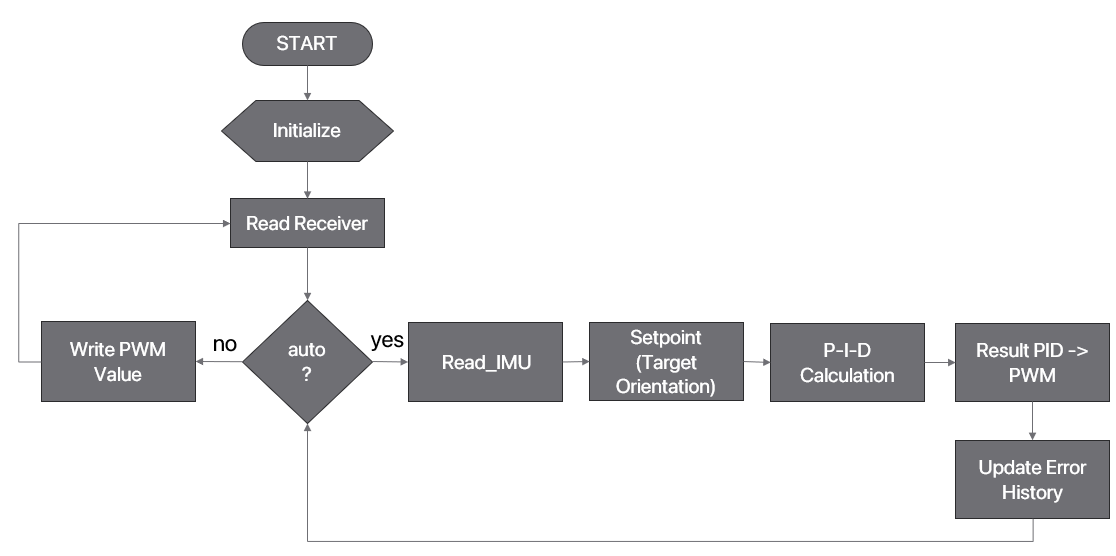
\includegraphics[width=1\linewidth]{pid3.png}
    \caption{Software design Flowchart}
    \label{fig:software}
\end{figure}
\end{frame}

%------------------------------------------------
\section{Testing of an Example PID}
\begin{frame}[fragile] % Need to use the fragile option when verbatim is used in the slide
\frametitle{Verbatim - 1}
\begin{example}[Roll angle test]
\begin{lstlisting}
The roll test results were given a peak disturbance of -17.52o and resulted in a steady-state error value of -1.00782, a rise time of 0.97 for the roll test was 0.1s, the setting time was 1.76, and the time required was 0.4s. The overshoot value was 4.65. Tuning results that produce Kp roll = 0.01, Ki roll = 1.3, and Kd roll = 0.01.
\end{lstlisting}
\cite{Susanto2024}
\end{example}
\end{frame}

%------------------------------------------------
\begin{frame}[fragile] % Need to use the fragile option when verbatim is used in the slide
\frametitle{Verbatim - 2}
\begin{example}[Pitch angle test]
\begin{lstlisting}
The results carried out on the pitch test were given a peak
disturbance of -21.93o and resulted in a steady-state error
value of -1.8, a rise time of 0.19, the time required for the pitch
test was 3.3s, the setting time was 2.47, and the time required
was 0.3s. The overshoot value was 3o and Tuning results that
produce Kp pitch = 0.3, Ki pitch = 0.01, Kd pitch = 0.02
\end{lstlisting}
\cite{Susanto2024}
\end{example}
\end{frame}

%------------------------------------------------
\begin{frame}[fragile] % Need to use the fragile option when verbatim is used in the slide
\frametitle{Verbatim - 3}
\begin{example}[Yaw angle test]
\begin{lstlisting}
The results of the yaw test were given a peak disturbance of -
14.01o and resulted in a steady-state error value of -3.1, a rise
time of 0.48, the time required for the yaw test was 0.6s, the
settling time was 4.65, and the time required was 4.5s. The
overshoot value was 3o. Tuning results that produce Kp yaw
= 1.3, Ki yaw = 0.01, Kd yaw = 0.01 
\end{lstlisting}
\cite{Susanto2024}
\end{example}
\end{frame}


%------------------------------------------------
\section{Citations \& Reference}

%------------------------------------------------


\begin{frame}[allowframebreaks]
\frametitle{References}
\nocite{
Widyantara2021,
Deswara2015,
Irmawan2018,
Prakoso2016,
Hartono2017,
Zakky2020}
\bibliographystyle{IEEEtran}
\bibliography{ref}

\end{frame}

%------------------------------------------------

\begin{frame}
\Huge{\centerline{Thank you}}
\end{frame}

%----------------------------------------------------------------------------------------

\end{document}